% !TEX root = ../thesis.tex
% !TEX spellcheck = en-US

\clearpage

\section{Explorative Experiments with Paragraph Dataset}

\section{Experiments with Sentence Dataset}

\subsection{Vector Space Models compared}


\todo{say why using the sentence dataset here}
\todo{reference jupyter notebook here}
% http://localhost:8888/notebooks/thesis/experiments/vector-space-models/Vector%20Space%20Models.ipynb#Setup

As Section~\ref{sec:vector-space-models} explains, a popular way to approach text classification and other tasks in natural language processing is to build a language model by creating explicit representations of the objects or entities to be processed in a vector space. Such vectors can be used as features for a learning algorithm. Depending on the representation they can also carry further meaning, such as to encode notions of similarity of associativity between the objects.

In order to determine effective vector space representations for the task of sentence classification, a set of experiments was carried out to study and compare different approaches. Each method was studied with regards to the effect of its hyper-parameters on effectiveness when producing an input space to different classifiers, but also time and memory requirements at training and inference time are taken into account \todo{actually discuss time and memory requirements}.

In order to compare the effectiveness for the sentence classification task as discussed in ?\todo{reference section here} each labelled document was transformed into a vector space representation using the different methods and then used for classification with a simple logistic regression classifier (\todo{link to logistic regression classifier explanation here}). Performance was then compared with regards to Matthews Correlation Coefficient for K classes (Section~\ref{par:Matthews Correlation Coefficient for K classes}) and the Accuracy \todo{link accuracy?} of the classifier.

\subsubsection{Baselines Classifiers: Uniform and Stratified Guessing}
\label{subs:baselines-classifiers}

As a baseline for comparing the performance of classification two different guessing strategies were used, namely uniform and stratified guessing.
Uniform guessing refers to a predictor that samples from the given classes assuming a uniform distribution whereas stratified guessing takes the label distribution in the data as the underlying probability distribution.
Then both methods just sample from these distributions to produce ``predictions'', while ignoring the actual input data. Both, uniform and stratified guessing achieve a Matthews Correlation Coefficient score of around 0 (averaged over 1000 runs) as expected for guessing strategies (see Section~\ref{subs:informedness-markedness-mcc}). On the other hand the accuracy for uniform guessing is around 0.16 which corresponds to $1/\text{K}$ for the K classes and around 0.26 for stratified guessing which reflects the skew of the label distribution.
Figure~\ref{fig:exp-vector-space-conf-matrix-guessing} shows the confusion matrices for these baseline variants in absolute and normalized form, revealing the properties of these guessing strategies.

\begin{figure}[h]
 % From http://localhost:8888/notebooks/thesis/experiments/vector-space-models/Vector%20Space%20Models.ipynb#Baseline:-Guessing-Strategies
    \centering
    \begin{subfigure}[b]{0.47\textwidth}
        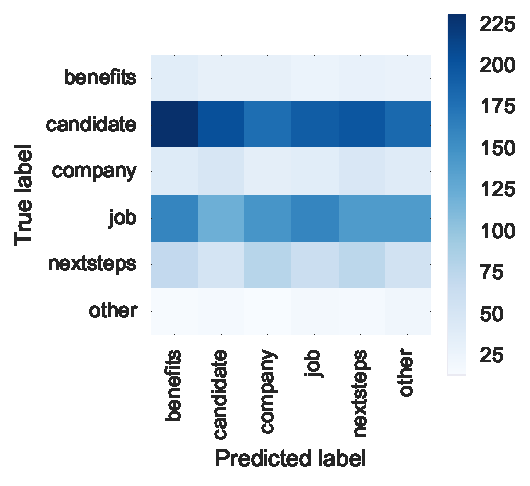
\includegraphics[width=\textwidth]{img/exp-vector-space-conf-matrix-guessing-uniform.pdf}
        \caption{Uniform, absolute}
    \label{fig:exp-vector-space-conf-matrix-guessing-uniform}
    \end{subfigure}
~
    %add desired spacing between images, e. g. ~, \quad, \qquad, \hfill etc.
    %(or a blank line to force the subfigure onto a new line)
    \begin{subfigure}[b]{0.48\textwidth}
        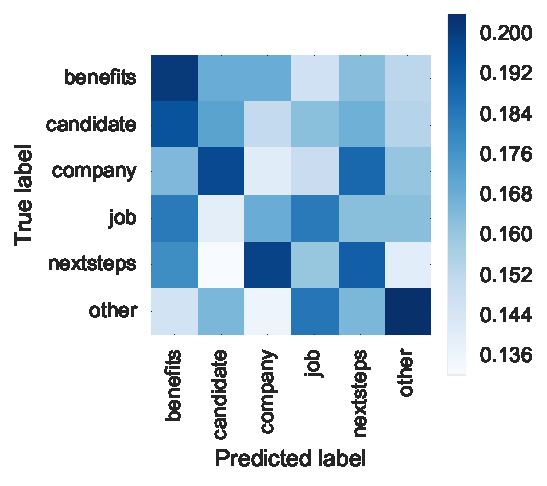
\includegraphics[width=\textwidth]{img/exp-vector-space-conf-matrix-guessing-uniform-normalized.pdf}
        \caption{Uniform, normalized}
      \label{fig:exp-vector-space-conf-matrix-guessing-uniform-normalized}
    \end{subfigure}
~
    \begin{subfigure}[b]{0.47\textwidth}
        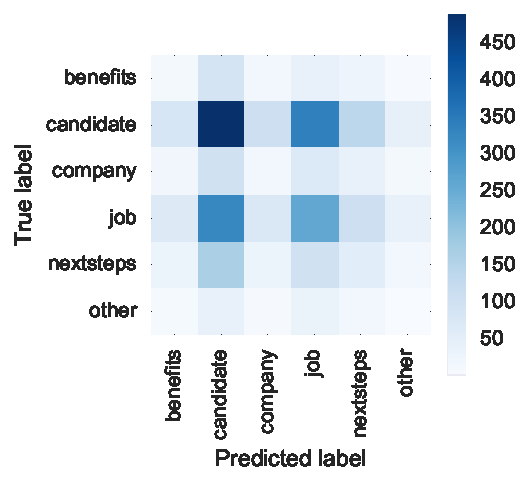
\includegraphics[width=\textwidth]{img/exp-vector-space-conf-matrix-guessing-stratified.pdf}
        \caption{Stratified, absolute}
      \label{fig:exp-vector-space-conf-matrix-guessing-stratified}
    \end{subfigure}
~
    %add desired spacing between images, e. g. ~, \quad, \qquad, \hfill etc.
    %(or a blank line to force the subfigure onto a new line)
    \begin{subfigure}[b]{0.48\textwidth}
        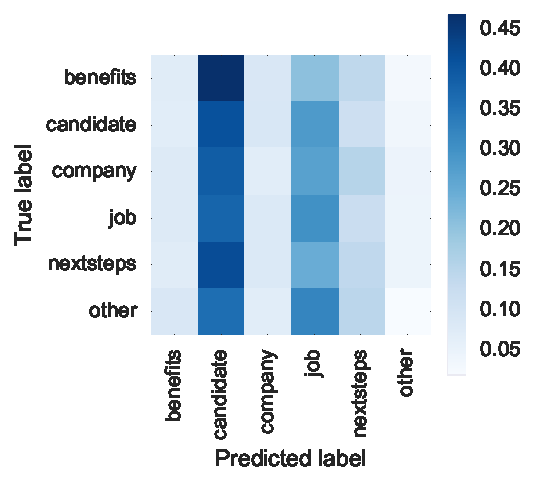
\includegraphics[width=\textwidth]{img/exp-vector-space-conf-matrix-guessing-stratified-normalized.pdf}
        \caption{Stratified, normalized}
      \label{fig:exp-vector-space-conf-matrix-guessing-stratified-normalized}
    \end{subfigure}
    \caption{Confusion matrices of uniform and stratified guessing strategies. }
\label{fig:exp-vector-space-conf-matrix-guessing}
\end{figure}

\subsubsection{N-gram Language Models}

The first class of language models that was investigated for the task of multi-class classification are N-gram models that were explained in Section~\ref{subs:n-gram-language-models}. As mentioned, in essence this type of model relies on simple statistics which makes for straightforward computation but at the same time comes at cost of expressiveness, especially in terms of temporal dependencies between words.

As N-grams models come in a variety of variants the most important ones were used as hyper-parameters to the model and a grid search was carried out over a wide range of combinations over these. The specific hyper-parameter settings are listed in Table~\ref{tab:ngram-parameters}. The grid search was optimized with regards to \emph{Matthews Correlation Coefficient} (see Section~\ref{par:Matthews Correlation Coefficient for K classes}) using 5-fold cross-validated with three standard classifiers: Logistic Regression and Naive Bayes and SVM.

\begin{table}[h]
  \begin{center}
  \begin{tabular}{ l l l}
    \toprule
    Hyper-Parameter & N-gram Type: Words & N-gram Type: Characters \\
    \midrule
    N-gram Range (Range) & [1,1], [1,2], [1,3], [2,3], [3,3] & [1,5], [1,10], [5,10], [5,15] \\
    Stop Words & English, None & N/A \\
    Vector Size (Size) & 10, 100, 300 & 10, 100, 300 \\
    IDF & Yes, No & Yes, No \\
    Norm & L1, L2, None & L1, L2, None \\
    Sub-linear TF & Yes, No & Yes, No \\
    \bottomrule
  \end{tabular}
  \caption{Parameter search space word and character level N-gram models}
  \label{tab:Ngram Parameters}
\end{center}
\end{table}

The 5 best results of these exhaustive grid searches can be seen in Table~\ref{tab:Ngram Grid Search} below.

\begin{table}[h]
  \begin{center}
  \begin{tabular}{ l l l l l l l l }
    \toprule
    Type & Range & Stop words & Size & IDF & Norm & Sub-linear TF & MCC Score \\
    \midrule
    Word & [1,1] & None & 300 & Yes &  & Yes & 0.689 \\
    Word & [1,1] & None & 300 & Yes &  & No & 0.687 \\
    Word & [1,1] & None & 300 & No &  & Yes & 0.682 \\
    Word & [1,1] & None & 300 & No &  & No & 0.682 \\
    Word & [1,1] & None & 300 & Yes & L2 & Yes & 0.68 \\
    % Word & [1,1] & None & 300 & Yes & L2 & No & 0.678 \\
    % Word & [1,2] & None & 300 & No &  & Yes & 0.677 \\
    % Word & [1,2] & None & 300 & Yes & L2 & Yes & 0.676 \\
    % Word & [1,2] & None & 300 & Yes & L2 & No & 0.675 \\
    % Word & [1,2] & None & 300 & No &  & No & 0.675 \\
    \midrule
    Word & [1,1] & None & 300 & No & & Yes & 0.659  \\
    Word & [1,1] & None & 300 & No & & No & 0.656 \\
    Word & [1,2] & None & 300 & No & & Yes & 0.655 \\
    Word & [1,2] & None & 300 & No & & No & 0.655 \\
    Word & [1,3] & None & 300 & No & & No & 0.65 \\
    % Word & [1,1] & None & 300 & Yes & L2 & Yes & 0.648 \\
    % Word & [1,1] & None & 300 & Yes & L2 & No & 0.648 \\
    % Word & [1,3] & None & 300 & No & & Yes & 0.648 \\
    % Word & [1,2] & None & 300 & Yes & L2 & No & 0.647 \\
    % Word & [1,2] & None & 300 & Yes & L2 & Yes & 0.646 \\
    \midrule
    Word & [1,1] & None & 300 & Yes & & Yes & 0.689 \\
    Word & [1,1] & None & 300 & Yes & & No  & 0.689 \\
    Word & [1,2] & None & 300 & Yes & & Yes & 0.677 \\
    Word & [1,2] & None & 300 & Yes & & No  & 0.677 \\
    Word & [1,3] & None & 300 & Yes & & Yes & 0.674 \\
    % Word & [1,3] & None    & 300 & Yes & & No  & 0.673 \\
    % Word & [1,1] & English & 300 & Yes & & Yes & 0.65 \\
    % Word & [1,1] & English & 300 & Yes & & No  & 0.65 \\
    % Word & [1,2] & English & 300 & Yes & & No  & 0.649 \\
    % Word & [1,2] & English & 300 & Yes & & Yes & 0.648 \\
    \bottomrule
  \end{tabular}
  \caption{Top 5 results of grid search over hyper-parameter space as listed in Table~\ref{tab:Ngram Parameters} using 5-fold cross-validated Logistic Regression (top), Naive Bayes (middle) and SVM (bottom) classifiers.}
\label{tab:Ngram Grid Search}
\end{center}
\end{table}

Across all classifiers the following results on the hyper-parameters can be observed:

\paragraph{Type}
\label{par:Type}
Words as the atomic unit for N-grams consistently lead to better results. This is understandable as the search space of combinations of characters is significantly larger than the search space of known words.

\paragraph{Range}
\label{par:Range}
There are slight differences to be observed between the three classifiers used, but with all three models the best performance is achieved using Unigrams. Also all of the top results across all classifiers include Unigrams in the model while extending the range towards bigrams or trigrams.

\paragraph{Stop Words}
\label{par:Stop Words}
None of the top results of the performed grid searches used stop words. This is interesting as using stop-words to remove hand-picked, highly frequent words that do not carry much meaning is common practice. It seems there is information carried within these stop words. Of course this outcome is also influenced by the particular stop-list used (see Section~\ref{subp:Stop words}).

\paragraph{Size (matters)}
\label{par:Size}
For the searched settings the largest vector dimensionality of 300 achieves the best performance. This is not surprising as higher-dimensional vectors can capture more information about N-gram occurrences. However in practice the vector size must be limited as it grows with the vocabulary -- potentially at an exponential rate if N-grams other than Unigrams are used. Also very high dimensionality often leads to decreased performance in terms of generalization of the model.

\paragraph{IDF}
\label{par:IDF}
There is no consensus between the classifiers on whether or not to weigh the N-gram frequencies by the \emph{inverse document frequency} (see Section~\ref{subp:TF.IDF weighting}). Thus it seems advisable to lead this parameter free for and evaluate both variants with a given classifier. For logistic regression however the performance differences are marginal and so the choice for this parameter seems somewhat arbitrary.

\paragraph{Norm}
\label{par:Norm}
Is seems that normalizing the vectors in most cases does not lead to any performance gains. Again this is an often recommended practice but here it does not seem to add any value to the model.

\paragraph{Sub-linear TF}
\label{par:Sub-linear TF}
Applying sub-linear TF (see Section~\ref{subp:Sublinear TF scaling}) does not seem to affect the results much and the choice of this parameter can hence be chosen almost arbitrarily as well, although here for all three classifiers applying it leads to a marginal improvement.

Table~\ref{tab:Ngram Grid Search Scores} shows the scores of each classifier using the best N-gram model. It is evident that here logistic regression actually performs best as it offers both, a good accuracy as well as the highest score for Matthews Correlation Coefficient.

\begin{table}[h]
  \begin{center}
  \begin{tabular}{ r | *3l | *3l }
    \toprule
     & \multicolumn{3}{c|}{Training} & \multicolumn{3}{|c}{Validation}\\
    Classifier & Accuracy & MCC & Accuracy & MCC \\
    \midrule
    Logistic Regression & 0.824 & 0.761 & 0.787 & 0.708 \\
    Naive Bayes         & 0.769 & 0.681 & 0.767 & 0.677 \\
    SVM                 & 0.835 & 0.681 & 0.786 & 0.700 \\
    \bottomrule
  \end{tabular}
  \caption{Performance of each best N-gram model with Logistic Regression and Naive Bayes on the validation data}
\label{tab:Ngram Grid Search Scores}
\end{center}
\end{table}

\begin{figure}[h]
    \centering
    \begin{subfigure}[b]{0.32\textwidth}
        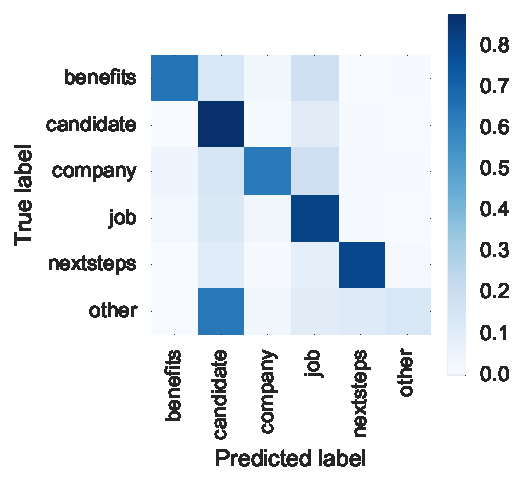
\includegraphics[width=\textwidth]{img/exp-vector-space-conf-matrix-logreg-normalized.pdf}
        \caption{Logistic Regression}
        \label{fig:exp-vector-space-conf-matrix-logreg-normalized}
    \end{subfigure}
    \begin{subfigure}[b]{0.32\textwidth}
        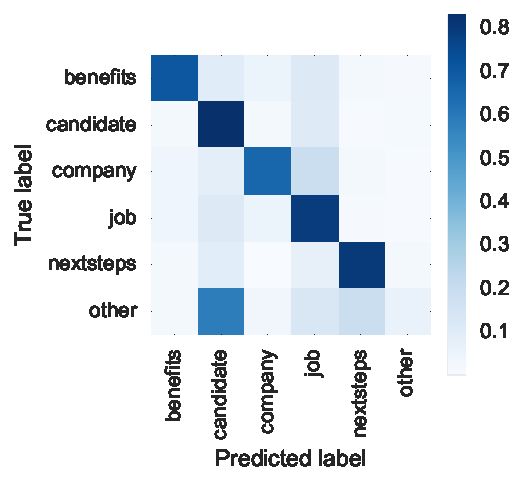
\includegraphics[width=\textwidth]{img/exp-vector-space-conf-matrix-naivebayes-normalized.pdf}
        \caption{Naive Bayes}
        \label{fig:exp-vector-space-conf-matrix-naivebayes-normalized}
    \end{subfigure}
    \begin{subfigure}[b]{0.32\textwidth}
        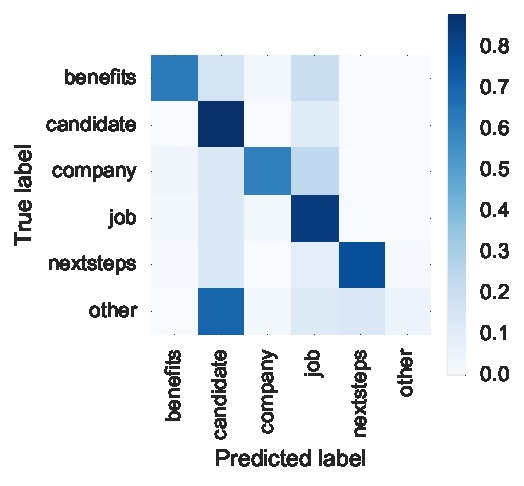
\includegraphics[width=\textwidth]{img/exp-vector-space-conf-matrix-svm-normalized.pdf}
        \caption{SVM}
        \label{fig:exp-vector-space-conf-matrix-svm-normalized}
    \end{subfigure}
    \caption{Confusion matrices all three classifiers using the best N-gram model found via cross-validated grid search. Both Naive Bayes as well as SVM show label bias towards the prevalent class \emph{candidate}.}
  \label{fig:exp-vector-space-conf-matrix-guessing}
\end{figure}

Figure~\ref{fig:exp-vector-space-ngram} shows projections of the of the constructed feature space using the best model that was optimized with Logistic Regression. This visualization shows the separability of the classes in this space. Especially the PCA projection here reveals that it is clearly possible to separate the classes until a certain point.

\begin{figure}[h]
    \centering
    \begin{subfigure}[b]{0.48\textwidth}
      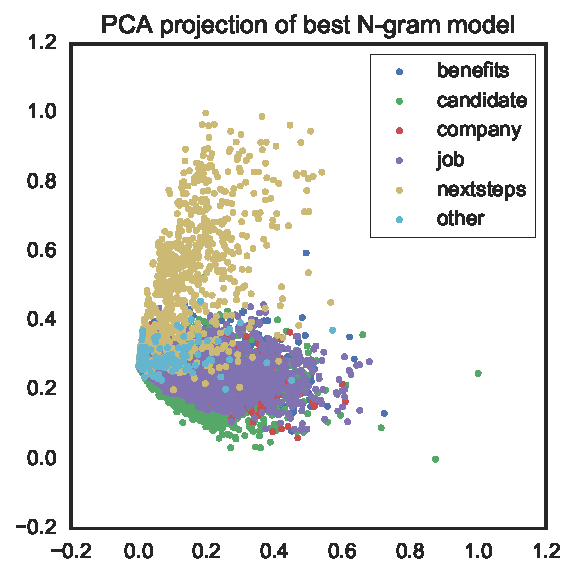
\includegraphics[width=\textwidth]{img/exp-vector-space-ngram-pca.pdf}
      \caption{PCA projection}
      \label{fig:exp-vector-space-ngram-pca}
    \end{subfigure}
    ~
    %add desired spacing between images, e. g. ~, \quad, \qquad, \hfill etc.
    %(or a blank line to force the subfigure onto a new line)
    \begin{subfigure}[b]{0.48\textwidth}
      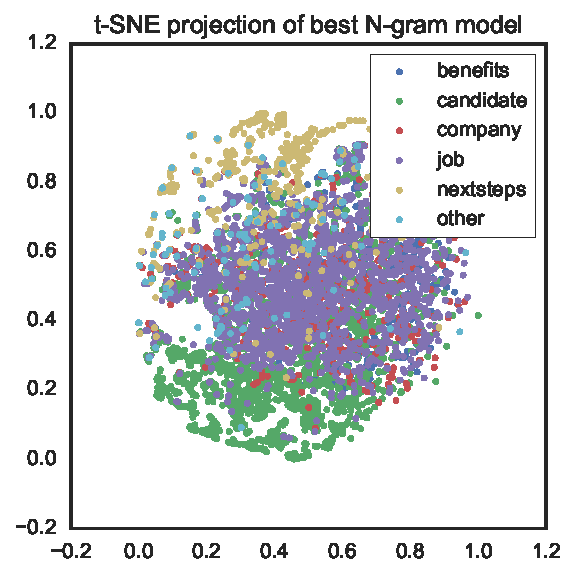
\includegraphics[width=\textwidth]{img/exp-vector-space-ngram-tsne.pdf}
      \caption{t-SNE projection}
      \label{fig:exp-vector-space-ngram-tsne}
    \end{subfigure}
    \caption{Document vectors produced by the best N-gram model (optimized w.r.t. Logistic Regression) projected onto the first 2 principal components (left) and project using t-SNE projection.}
  \label{fig:exp-vector-space-ngram}
\end{figure}

\subsubsection{Bag-of-Means -word2Vec averaged *}



\subsubsection{Doc2Vec --- Distributed representations of documents *}

\paragraph{Vector Size *}

\paragraph{Frequent word Sub-Sampling *}

\paragraph{Hierarchical Sampling *}

\paragraph{Negative Sampling *}

\paragraph{Window Size *}

\paragraph{CBOW versus PM-DV *}

\paragraph{Evaluating the best hyper-parameter setting *}

\subsubsection{Doc2Vec using pre-initialized weights *}

\subsubsection{Doc2Vec using context sentences *}

\subsubsection{Results and Discussion *}




\subsection{Finding the best Classifier using Vector Space Models}

\subsection{Advanced and experimental approaches}

\subsubsection{Inversion of Distributed Language Representations}

\subsubsection{LSTM Multi-task learner}
\label{subs:LSTM Multi-task learner}
